\author{Студенти: Светозар Иковић, Јелена Јеремић \\ Ментор: проф. др Ненад Митић}
\documentclass[10pt, a4paper]{article}

\usepackage{csvsimple}
\usepackage{changepage}
\usepackage{cclicenses}
\usepackage{pbox}
%\usepackage[document]{ragged2e}
\usepackage{xcolor,colortbl}
\usepackage{url}
\usepackage[T2A]{fontenc}
\usepackage[utf8]{inputenc} % make weird characters work
\usepackage{graphicx}
\usepackage{geometry}
\usepackage{amsmath}
\usepackage[justification=centering]{caption}
\usepackage{enumitem}

\graphicspath{{slike/}}

\usepackage[unicode]{hyperref}
\hypersetup{colorlinks,citecolor=black,filecolor=green,linkcolor=blue,urlcolor=blue}

\usepackage[english,serbianc]{babel}

\usepackage{datetime}
\newdateformat{specialformat}{\twodigit{\THEDAY}.\twodigit{\THEMONTH}.\THEYEAR.}
\date{\specialformat\today}

\usepackage{listings}
\usepackage{float}
\restylefloat{table}
\usepackage[natbib=true, style=authoryear, labelnumber]{biblatex}
\renewbibmacro{in:}{}
\addbibresource{main.bib}

\DeclareLanguageMapping{serbianc}{english-apa}
\DefineBibliographyStrings{english}{%
  andothers = {\textbf{et al}\adddot}
}

\DefineBibliographyExtras{english}{%
  \renewcommand*{\finalnamedelim}{\addcomma\addspace}%
}

\DeclareNameAlias{default}{first-last}
\renewcommand*{\revsdnamepunct}{}

\DeclareFieldFormat{labelnumberwidth}{[#1]}
\defbibenvironment{bibliography}  % from numeric.bbx
  {\list
    {\printtext[labelnumberwidth]{%
      \printfield{prefixnumber}%
      \printfield{labelnumber}}}
    {\setlength{\labelwidth}{\labelnumberwidth}%
        \setlength{\leftmargin}{\labelwidth}%
        \setlength{\labelsep}{\biblabelsep}%
        \addtolength{\leftmargin}{\labelsep}%
        \setlength{\itemsep}{\bibitemsep}%
        \setlength{\parsep}{\bibparsep}}%
        \renewcommand*{\makelabel}[1]{\hss##1}}
  {\endlist}
  {\item}


\definecolor{LightCyan}{rgb}{0.88,1,1}
\definecolor{LightYellow}{rgb}{1.0, 0.98, 0.8}
\lstset{}

\begin{document}
\newpage
\title{Кластеровање мононуклеарних ћелија периферне крви \\ \small{Семинарски рад у оквиру курса Истраживање података 2 \\ Математички факултет}}
\author{Студенти: Светозар Иковић, Јелена Јеремић \\ Ментори: проф. др Ненад Митић, Александар Вељковић}


\maketitle
\renewcommand\abstractname{Сажетак}
\renewcommand\contentsname{Садржај}
\renewcommand{\figurename}{Слика}

\begin{abstract}
Мононуклеарне ћелије периферне крви су изузетно битна компонента имуног система јер могу изазвати реакцију на ,,уљезе'' који уђу у тело човека или на већ постојеће ћелије које су се трансформисале у ћелије канцерогеног типа. Из тог разлога се често користе при истраживањима у областима: имунологије, инфективних болести, хематолошким малигностима, развоју вакцина, трансплатација и токсикологије. Лако се прикупљају, преносе и складиште, при чему постоје разрађене процедуре руковања којима се чува употребљивост узорака. Прецизним и успешним процесирањем и анализом ових ћелија могу се тестирати имуне реакције и стећи дубље разумевање имуног система што се касније може применити на третмане и лечења болести код људи. Свака подгрупа ових ћелија има јединствен образац испољавања тј. експресије гена. Унутар тих група, при поређењу појединачних ћелија, могу се дешавати одређена мања или већа одступања у експресији гена у зависности од старости и фазе развоја ћелија, места настанка одређених подгрупа ћелија, али и тога да ли се пореде здрава или болесна ћелија. Метод једноћелијске транскриптомије је нова технологија која омогућава генерисање профила експресије гена великог скупа ћелија у ком можемо видети профил сваке ћелије појединачно. На основу профила ћелије се могу груписати према сличности и уочити које су ћелије здраве, а које не. Један од најчешће коришћених метода којима се ћелије групишу на основу сличности профила је кластеровање. У овом раду смо упоредили неколико алгоритама кластеровања који су се у неким ранијим радовима показали као веома успешни и навели који су се над нашим скупом података најбоље показали.
\end{abstract}

\newpage
\tableofcontents
\newpage

\setlength{\parskip}{0.5em}

\section{Увод}
\label{sec:uvod}

Периферна крв је крв која циркулише кроз тело човека. Састоји се од црвених крвних зрнаца (еритроцита), белих крвних зрнаца (леукоцита) и крвних плочица (тромбоцита). Разликује се од крви која циркулише искључиво унутар јетре, слезине, коштане сржи и лимфног система. \textbf{Мононуклеарне} ћелије (PBMC\footnote{PBMC (eng.~{\em peripheral blood mononuclear cell})}) чине све оне ћелије периферне крви које имају округло једро. Бела крвна зрнца садрже округло једро, док еритроцити и тромбоцити немају једро.  Бела крвна зрнца се деле на лимфоците и моноците.

Код људи, лимфоцити, а након њих моноцити, сачињавају највећи део PBMC ћелија. Најмањи део PBMC ћелија сачињавају дендритске ћелије. Лимфоцити припадају роду лимфоидних ћелија и основа су адаптивног имунског система. Моноцити и дендритске ћелије припадају роду мијелоидних ћелија које имају веома широк спектар улога, попут урођеног имунитета, адаптивног имунитета и згрушавања крви. Лимфоцити се даље деле на три главне подгрупе: Т ћелије (TC), Б ћелије (BC) и ћелије убице (NK). Оне се могу лако идентификовати због великог једра. Ове подгрупе лимфоцита се по облику не разликују, већ само по функцији коју обављају:

\begin{itemize}
\item\textbf{Б ћелије} су одговорне за хуморални имунитет који се односи на активност имуног система против екстрацелуларних патогена и њихових токсина. Настају у коштаној сржи и чине од 5\% до 15\% људског PBMC-а
\item\textbf{Т ћелије} су одговорне за ћелијски имунитет коме је главна мета инфицирана ћелија домаћина. Оне сазревају у тимусним тимоцитима (ћелијама присутним у тимусу) и чине од 40\% до 70\% људског PBMC-а
\item\textbf{Ћелије убице} су посебна група које имају улогу у одбрани организма против вируса и туморских ћелија тј. спречавају размножавање ненормалних ћелија. Оне чине од 5\% до 10\% људског PBMC-а
\end{itemize}

\textbf{Моноцити} су посебна врста леукоцита, крупне ћелије које поседују фагоцитне способности (уништавање бактерија и других страних тела). Оне чине од 10\% до 30\% људског PBMC-а.
\textbf{Дендритске ћелије} настају у коштаној сржи и одликују их разгранати цитоплазматски продужеци. Оне патролирају телом тражећи бактерије, вирусе или опасне токсине. Потом путују до лимфних чворова или слезине где подстичу друге ћелије имуног система (углавном Б и Т ћелије) да крену у напад и униште их.

Анализа експресије гена унутар ћелија омогућава детаљан увид у начин функционисања ћелија у нормалном стању или у неким патолошким стањима. \cite{celije}\cite{transkriptomija} Тиме се могу правити поређења здравих и болесних ћелија и лако уочити присуство неких болести. \textbf{Метод једноћелијске транскриптомије} (SCT\footnote{SCT (eng.~{\em single-cell transcriptomics}) или scRNA-seq (eng.~{\em single-cell RNAsequencing})}) тј. једноћелијско РНК секвенцирање омогућава пребројавање испољавања информационе РНК (\textbf{експресије гена}) унутар појединачних ћелија. Овиме добијамо транскриптомски профил одређене групе ћелија где је за сваку ћелију анализирану приказан транскриптом тј. број испољавања сваког гена у њој. Овај метод се до сад показао као један од најпоузданијих јер успева да представи и очува испољавање сваког гена унутар појединачне ћелије (методи пре овога су углавном највише могли дати неки просек испољених гена на основу посматраног узорка ћелија). 

Са друге стране, SCT има одређених ограничења због честог присуства лажно-негативних резултата који као резултат дају ретке матрице (са великим бројем нула гена), али и лажно-позитивних резултата који настају због потребе умножавања РНК ради секвенцирања што доводи до неједнаке покривености транскрипта (неки значајни делови се приликом умножавања могу изгубити). На присуца дрство лажно-позитивних резултата утичу и различити начини претпроцесирања појединачних ћелија: третирање додатним хемикалијама ради издвајања сваке ћелије, сортирање ћелија или издвајања одређених гена.

На основу профила ћелије можемо груписати и тиме разликовати здраве од болесних ћелија. Један од метода ненадгледаног учења који се до сад у већој мери показао као доста успешан је кластеровање. Међутим и овај метод груписања има својих мана: усред могућих грешака због осетљивости материјала при прављењу профила, неке здраве или болесне ћелије могу упасти у погрешне кластере и често је након формирања кластера потребна додатна ручна обрада кластера. Под овим се подразумева да је потребно познавати тачан број сваке подгрупе ћелија како би се касније могао проверити квалитет формираних кластера тј. да ли су очекиване ћелије груписане заједно и колико су кластери чисти тако да присуство ћелија за чији тип нисмо сигурни овде не би било пожељно.

Такође се као проблем јавља {\em,,проклетство димензионалности''} где због присуства великог броја гена (тј. високе димензионалности) удаљености између кластера постају мање и кластери делују сличније. Циљ овог рада је да се са неколико различитих алгоритама покуша прављење што прецизнијих кластера тј. група ћелија који се разликују према експресији гена. Поред прављења ових ненадгледаних модела, могуће је помоћу вештачких неуронских мрежа изградити полунадгледане моделе, са бољим учинком, али они неће бити тема овог рада.

\section{Скупови података}
\label{sec: naslov2}

Обрађени скуп података чини 18 датотека (профила) преузетих из базе \textbf{GEO} ({\em Gene Expression Omnibus})\footnote{\url{https://www.ncbi.nlm.nih.gov/}}. Свака датотека у свом називу садржи датум кад је објављена и коју групу или подгрупу ћелија садржи у себи. Неке од датотека у свом називу додатно садрже јединствену ознаку узорка (облика GSMброј) као и хемикалије којима је узорак третиран, молекули и протеини које ћелије испољавају, редни број донатора или редни број експеримента. Сви узорци су већ прочишћени и имају исти број гена (30688) у истом редоследу, али је број ћелија у сваком од узорака другачији. Редове чине гени, а ћелије су распоређене у колоне. Поље (i, ј) унутар сваке табеле носи информацију колико је у ћелији \textbf{ј} регистровано испољавања тј. транскрипата гена \textbf{i}.

Информације су дате у виду целих бројева, од нуле па навише. Све матрице су врло ретке тј. већи део поља као вредност имао је уписану нулу. Гени су унутар сваке датотеке већ били преименовани према речнику GRCh38 (hg38) Референтног конзорцијума за геном.  Профили добијени су поређени са профилима добијеним на основу обраде узорака преузетих из других извора (Broad Institute\footnote{\url{https://singlecell.broadinstitute.org/single\_cell}}, 10X\footnote{\url{https://support.10xgenomics.com/single-cell-gene-expression/datasets}}) и приликом поређења уочене су неке несагласности са осталим профилима. Разлог постојања несагласности је додатно третирање биолошког материјала различитим хемикалијама. Додатна обрада материјала може изазвати одређену количину промена у експресији гена чиме се одступа од стварног стања. 

На пример, након третирања различитим хемикалијама два иста узорка од једне особе, та два узорка могу деловати различитије него да нису била додатно третирана хемикалијама. Слично се може десити са два узорка од две различите особе, где ће узорци деловати сличније након третирања хемикалијама.

Опис датих узорака:
\begin{itemize}
\item\textbf{Б ћелије: }Два узорка постоје са ћелијама овог типа. Главна разлика је модел машине којим је секвенцирање вршено: у узорку \textbf{GSM3258348} секвенционирано је 1760 ћелија HiSeq X Ten моделом, док је у узорку \textbf{GSM3258346} секвенционирано 26 ћелија Illumina MiSeq моделом
\item\textbf{Дендритске ћелије:} Два узорка постоје са ћелијама овог типа. Као и у случају са Б ћелијама и овде је главна разлика модел машине којим је секвенцирање вршено: у узорку \textbf{GSM3258347} секвенционирано је 2397 ћелија HiSeq X Ten моделом, док је у узорку \textbf{GSM3258345} секвенционирано свега 48 ћелија Illumina MiSeq моделом
\item\textbf{Моноцити: }Два узорка постоје са ћелијама овог типа, разликују се према томе што потичу од два различита донатора. Узорак \textbf{GSM2773408} садржи 425 ћелија, а \textbf{GSM2773409} садржи 431 ћелију
\item\textbf{НК ћелије: }Само један узорак ћелија овог типа је дат, са 309 ћелија унутар овог узорка
\item\textbf{Т ћелије: }Највећи број узорака (11) садржи ћелије овог типа. Узорци се разликују према томе коју подгрупу Т ћелија садрже:

\begin{itemize}
\itemУзорак \textbf{20190108\_iNKT} садржи подгрупу Т ћелија које деле карактеристике НК и Т ћелија и представљају мост између адаптивног (стеченог) имуног система и урођеног имуног система. Ова подгрупа Т ћелија спада у врсту Т ћелија које изазивају брз одговор имуног система. У овом узорку је 325 ћелија
\itemУзорак \textbf{20190108\_MAIT} садржи подгрупу која, такође, изазива веома брз одговор имуног система. За ову врсту се касније открило у односу на остале, прве објаве о овој врсти датирају из 2009. Сматра се да играју битну улогу код аутоимуних болести, попут мултипле склерозе и упалних болести црева. Узорак садржи 382 ћелије
\itemУзорак \textbf{GSM3478792} садржи 4486 нормалних Т ћелија
\itemУзорак \textbf{GSM3430548} садржи 1247 супресорских Т ћелија, познатијих и као регулаторне Т ћелије. Ћелије унутар овог узорка спадају у специфичну подгрупу {\em IL-10 FOXP3-} регулаторних Т ћелија. FOXP3 представља транскрипциони фактор тј. протеин који ове ћелије изражавају и може се користити за лакшу идентификацију ове врсте ћелија. IL-10 је супресивни молекул (цитокин) који ћелије луче
\itemУзорак \textbf{20190108\_CD4\_T} садржи 222 помоћних Т ћелија
\itemУзорак \textbf{GSM3209407} садржи 965 помоћних Т ћелија
\itemУзорак \textbf{GSM3209408} су подгрупа меморијских Т ћелија. Ова врста опстаје дуго времена након савладавања инфекције чиме се меморише активност на све прошле инфекције. Садржи 435 ћелија
\itemУзорак \textbf{20190108\_CD8} представља подгрупу цитоксичних Т ћелија. Садржи 310 ћелија
\itemУзорак \textbf{GSM3087629} је подгрупа цитоксичних Т ћелија третираних метанолом у току фазе припреме за секвенционирање. Садржи 4753 ћелија
\itemУзорци \textbf{20190108\_Vd1} и \textbf{20190108\_Vd2} садрже малу подгрупу Т ћелија познатих као {\em Гама делта} Т ћелије. Први узорак садржи 284, а други узорак садржи 204 ћелије
\end{itemize}
\end{itemize}

\section{Претпроцесирање и подела тока рада}
\label{subsec: podnaslov2}
Цео рад био је подељен на два тока. Обрада података у оквиру првог тока подразумевала је кластеровање ћелија без избацивања иједног гена тј. реда из датих матрица. Обрада другог тока подразумевала је избацивање свих нула гена тј. редова који су садржали само нуле као вредности. Циљ раздвајања рада на ова два тока био је како би се тестирало да ли присуство нула гена има икаквог утицаја на формирање кластера. У оба тока рада нису избацивани гени ако постоји барем једна ћелија унутар узорка где се ген испољава. Разлог овоме је што због врло осетљиве обраде узорака приликом прављења профила, може се десити да испољавање гена грешком није уочено у осталим ћелијама. Такође, нула не означава да гена у ћелији нема него да се није детектовало његово испољавање, тако да очување гена који су се слабо испољили може бити од користи.

Други део припреме података представљало је транспоновање матрица унутар датотека како би ћелије чиниле редове матрице, а гени колоне. Измене које су паралелно направљене је да су редови тј. ћелије преименовани у облику {\em,,СкраћеноИмеДатотеке\_редниБројРеда''}. Разлог преименовања је како би се касније при спајању података по редовима из различитих датотека, лако могло разазнати из које датотеке је потекао који ред. Додатна провера датотека након транспоновања није била неопходна јер, као што је већ напоменуто, у свим датотекама је редослед и број гена идентичан.

Трећи део припреме била је логаритамска трансформација података како би се постигле боље перформансе алгоритама.

\subsection{Модули и технике коришћенe за обраду података}
\label{subsec: podnaslov3}

Коришћен је програмски језик {\em Python} уз модул {\em sklearn} и софтверски оквир {\em scanpy}. Сваки алгоритам је испробан више пута уз различито подешавање параметара тог алгоритма како би се постигли што чистији и раздвојенији кластери. У оба тока рада нису избацивани гени ако постоји барем једна ћелија унутар узорка где се ген испољава. Зарад визуелизације, коришћенa је техника \textbf{UMAP} која је улазне податке представљала у две димензије.

\subsubsection{Scanpy}
\label{subsec: podpodnaslov1}

Scanpy ({\em Single-Cell Analysis in Python})\footnote{Више о софтверском оквиру можете погледати овде: \url{https://scanpy.readthedocs.io/en/stable/}} је скалабилни скуп алата за анализу профила добијеног једноћелијском експресијом гена. \cite{scanpy} Садржи методе за препроцесирање, визуелизацију, кластеровање као и многе друге напредне технике корисне истраживачима за анализу профила. Имплементиран је у Python-у и нуди ефикаснију обраду скупова са више од милион ћелија у односу на раније развијене алате. У односу на раније развијене алате, обрада података овде је убрзана од 5 до 90 пута (у зависности од тога са којим алатима се пореди) што значи да око 100000 ћелија се може обрадити у року од неколико секунди.

Scanpy нуди и генеричку класу за обраду означених матрица – {\em AnnData}, која је и коришћена у раду јер нуди скалабилне методе за праћење самих података као и додатних информација о њима. Класа {\em AnnData} из пакета anndata\footnote{Више о пакету овде: \url{https://anndata.readthedocs.io/en/latest/}} матрице података посматра као означене - чува одвојено од података информације о узорцима (ћелијама тј. именима редова матрице) и о атрибутима (генима тј. колонама матрице). Податке унутар саме матрице посматра засебно, тако да ако би у матрицу било потребно поставити нове податке, а да имена редова и колона остану иста, подаци се могу лако сменити јер се посматрају раздвојено. Сви алати Scanpy-а су изграђени да раде само са оваквим матрицама и пошто се очекује да и сваки алат ради искључиво са оваквим матрицама, лако се могу додавати нове функционалности за алате, без бриге о томе какав формат података морају подржати.

Scanpy за репрезентацију, рачунање и чување суседа међу инстанцама користи графове. Једном израчунат граф се касније користи у свим осталим методама где су информације о суседима потребне тиме избегавајући изнова скупа рачунања и репрезентацију података. Овиме омогућава брже рачунање и налажење најближих суседа него пакети који се најчешће користе за ово. 

\subsubsection{UMAP}
\label{subsec: podpodnaslov2}

UMAP ({\em Uniform Manifold Approximation and Projection})\footnote{Више о овој техници можете погледати овде: \url{https://umap-learn.readthedocs.io/en/latest/index.html}} је новија техника нелинеарне димензионе редукције. Алгоритам који се до сад најчешће користио у ове сврхе је \textbf{tSNE}. tSNE се истиче у својој ефикасности при наглашавању локалне структуре унутар података. Проблем код података као што су ћелије и екпсресије гена у њима је што наглашавање локалне структуре може довести до репрезентације појединачних ћелија као засебних кластера. Због тога се губи на очувању глобалне структуре података, а уз то tSNE са порастом димензија и броја инстанци за кластеровање захтева много дуже време обраде. \textbf{UMAP је развијен са циљем да се глобална структура очува што боље и што верније представи, а сва та обрада се врши за много краћи временски рок}. Примера ради, UMAP може пројектовати 784-димензионални скуп података са 70000 инстанци за мање од три минута, док tSNE алгоритму ће бити потребно око 45 минута.

UMAP је базиран на Римановој геометрији и алгебарској топологији. \cite{understanding_umap} Алгоритам се састоји из две фазе - конструисања расплинуте (eng. ~{\em fuzzy}) тополошке репрезентације, а потом оптимизације нискодимензионалне репрезентације како би се што верније представила и очувала оформљена расплинута репрезентација. За добијање расплинуте репрезентације прве фазе, посматрају се само најближи суседи за сваку тачку. Суседе можемо очитати из матрице суседа, а алгоритму наводимо колико суседа желимо да гледа. Резултат је практичан и скалабилан алгоритам који ефикасно ради са великим подацима. Укратко речено, конструише се високодимензионални граф података, а потом се оптимизује нискодимензионални граф, који се користи за репрезентацију, како би структура опстала што сличнија.

Два параметра која су најбитнија да се задају алгоритму су \textbf{број суседа} ({\em n\_neighbors}) и \textbf{минимална дистанца} ({\em min\_dist}). \textbf{Број суседа} је број који даје потребан (приближан) број најближих суседа који су потребни за конструкцију високодимензионалног графа. Важност овог параметра лежи у томе што он контролише како алгоритам балансира између наглашавања локалне и глобалне структуре. Ниже вредности доводе до наглашавања локалне структуре, а више до наглашавања глобалне структуре уз губитак нагласка на детаље. \textbf{Минимална дистанца} је број који задаје најмању дистанцу која може постојати између тачака при репрезентацији у нискодимензионалном простору. Параметар контролише колико густо алгоритам пакује тачке (инстанце) заједно. 

Ниже вредности доводе до густих репрезентација тј. тачке које су суседи представљене су веома близу једна другој. Веће вредности доводе до ,,лабавије'' репрезентације тј. суседи нису веома густо представљени чиме се чува и боље представља шира тополошка структура.

Scanpy се за налажење најближих суседа веома ослања на UMAP који користи како би ефикасније проценио повезаност две инстанце. У Scanpy постоји библиотека која за репрезентацију графа суседа у захтеваном броју димензија користи UMAP.

\section{Кластеровање и поређење резултата}
\label{sec: naslov3}
Могућност дефинисања типа ћелија кроз ненадгледано учење на основу сличности транскриптома једна је од најмоћнијих примена SCT-а. \cite{spektralno1} Кластеровање се до сад показало као један од успешнијих метода анализе профила. Међутим услед велике количине података, јединствен процес кластеровања оваквих података не постоји - различити алгоритми могу дати резултате који се међусобно изузетно разликују. Циљ је пронаћи групе ћелија тако да оне које су заједно груписане су међусобно што сличније, а да ћелије из различитих група буду што различитије. Дакле, растојања унутар кластера желимо минимизовати, а растојања између два и више кластера треба максимизовати што је више могуће.
Мењајући вредности параметара алгоритама који се примењују, можемо наводити алгоритам на број кластера који очекујемо. Испробане су технике партиционог кластеровања, а међу њима алгоритми засновани на репрезентативним тачкама, густини и графовима. У циљу формирања што прецизније матрице суседа испробане су разне метрике простора.

\subsection{Идеална слика}
\label{subsec: podnaslov4}
Пре примене било ког алгоритма, визуелизован је ,,идеалан модел'' података који представља расподелу ћелија у две димензије. За визуелизацију коришћена је техника UMAP, a боје нам говоре којем типу ћелија припада која тачка са цртежа.

\begin{figure}[h]
    \centering
    \captionsetup{justification=centering}
    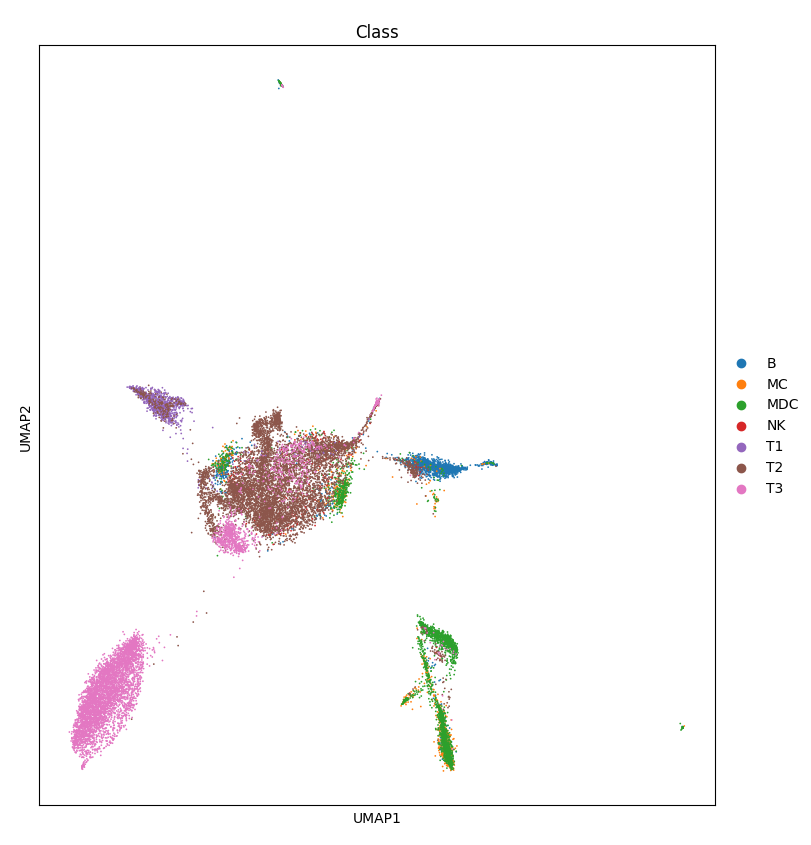
\includegraphics[width=0.7\textwidth]{umap1.png}
    \caption{Визуелизација UMAP са метриком L2 и са параметром број суседа подешен на 110}
    \label{fig:gustina2}
\end{figure}

\subsection{Алгоритми засновани на репрезентативним тачкама}
\label{subsec: podnaslov5}
Неки од најпопуларнијих алгоритама су они засновани на налажењу најрепрезентативнијих центара за сваки кластер. Ова метода кластеровања налази {\em К} најбољих центара како би улазне податке поделио на {\em К} кластера. Центар може представљати \textbf{центроид}\footnote{израчуната аритметичка средина позиција свих тачака у том кластеру} или \textbf{медоид}\footnote{тачка из улазних података чији просек различитости од осталих тачака у кластеру је минималан}.

Један од алгоритама из ове групе је \textbf{\em KMeans} (K средина). Он за центре кластеровања налази центроиде са циљем да минимизује еуклидску дистанцу између тачака кластера и самог центроида кластера. Тако се кроз више итерација формирају кластери у којима се тачка додели оном кластеру од чијег центра је најмање удаљена. \cite{kmeans}

Стандардни K средина алгоритам користи Лојдов алгоритам који је скалабилан и може се користити за кластеровање велике количине података. Уз то му је и временска комплексност ниска ({\em O(NKD)}, N = број тачака које кластерујемо, K = број кластера, D = број димензија).Мана алгоритма је осетљивост на присуство елемената ван граница и шума. Такође, неопходно је проследити жељени број кластера К, тако да је потребна барем нека основна претпоставка о броју кластера како би се алгоритам могао користити. Лојдов алгоритам, иако погодан за рад са већом количином података, спада у похлепне алгоритме и има тенденцију налажења локалних минимума уместо глобалних. Овај проблем се може превазиђи већим бројем извршавања алгоритма над подацима, сваки пут са другачијим параметрима. Међутим, већи проблем прави чињеница да се Лојдов алгоритам користи за проналажење равномерно распоређених скупова тачака и тежи ка томе да сви скупови буду скоро исте величине што може довести до тога да се неки битни скупови ретких типова ћелија прекрију неким већим скупом ћелија. Добијени резултати се разликују у зависности од прослеђеног броја очекиваних кластера.
\begin{figure}[H]
    \centering
    \captionsetup{justification=centering}
    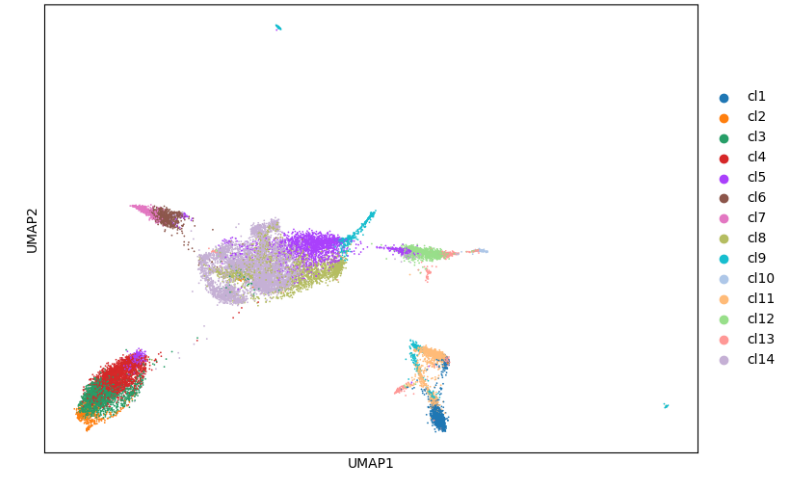
\includegraphics[width=\textwidth]{kmeans_euc.png}
    \caption{Четрнаест кластера KMeans са Минковски метриком}
    \label{fig:gustina2}
\end{figure}

\begin{figure}[H]
    \centering
    \captionsetup{justification=centering}
    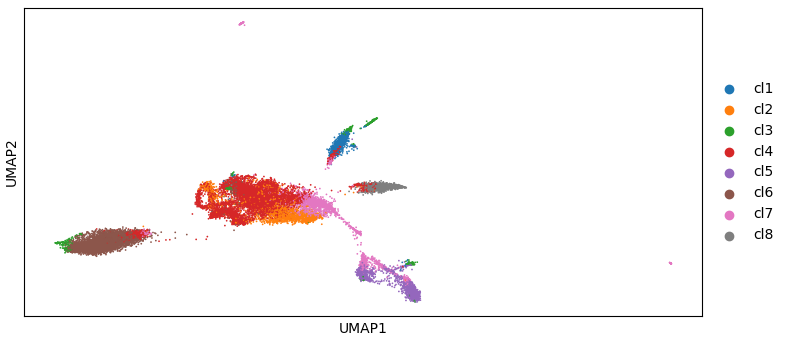
\includegraphics[width=\textwidth]{kmeansmink.png}
    \caption{Осам кластера KMeans са Минковски метриком}
    \label{fig:gustina2}
\end{figure}
\newpage
\subsection{Алгоритми засновани на густини}
\label{subsec: podnaslov6}
Код алгоритама кластеровања који су засновани на густини, кластери се дефинишу као регије велике густине тачака у простору. Регије са малом густином се третирају као шум или елементи ван граница и они раздвајају регије велике густине.

Битна два параметра алгоритма су \textbf{максимална дистанца} између две тачке да би се за њих сматрало да су суседи и \textbf{број инстанци} који морају чинити суседе неке тачке како би та тачка била проглашена за центар неког кластера. Тачке се тако деле на три категорије – \textbf{тачке језгра} што представљају све тачке на растојању мањем од задате максималне дистанце (тј. припадају језгру неке тачке и онда се смештају у исти кластер као и тачка језгра), \textbf{тачке на граници} које ће припасти истом кластеру као и тачка језгра на чијој се граници налазе и \textbf{тачке шума} које не припадају кластеру. Алгоритам за сваку тачку скупа врши проверу да ли припада неком кластеру и ком. Веома је погодан и врло ефикасно (временска сложеност {\em О(nlogn)}) ради за детекцију кластера било којег облика (дакле не морају бити само кластери кружног облика). Међутим из овога можемо видети да је мана овог алгоритма што претпоставља да сви кластери имају сличну густину, што значи да ако имамо кластере са великом густином тачака, кластери који имају мању густину ће бити означени само као скуп тачака који не припада ниједном кластеру.

Алгоритам је испробан и на овим подацима, али је у односу на остале дао најлошије резултате. У зависности од модификације два раније поменута параметра, подаци су или били скоро сви стављани у један велики кластер, а мањи број је био проглашен за аномалију или су готови сви подаци били проглашени као аномалије, а само је мањи део био стављен у један кластер. Мењане су и метрике које се користе да би се рачунале удаљености тачака, међутим ни то није допринело бољим резултатима.
% https://tex.stackexchange.com/questions/35125/how-to-use-the-placement-options-t-h-with-figures
\begin{figure}[H]
    \centering
    \captionsetup{justification=centering}
   % 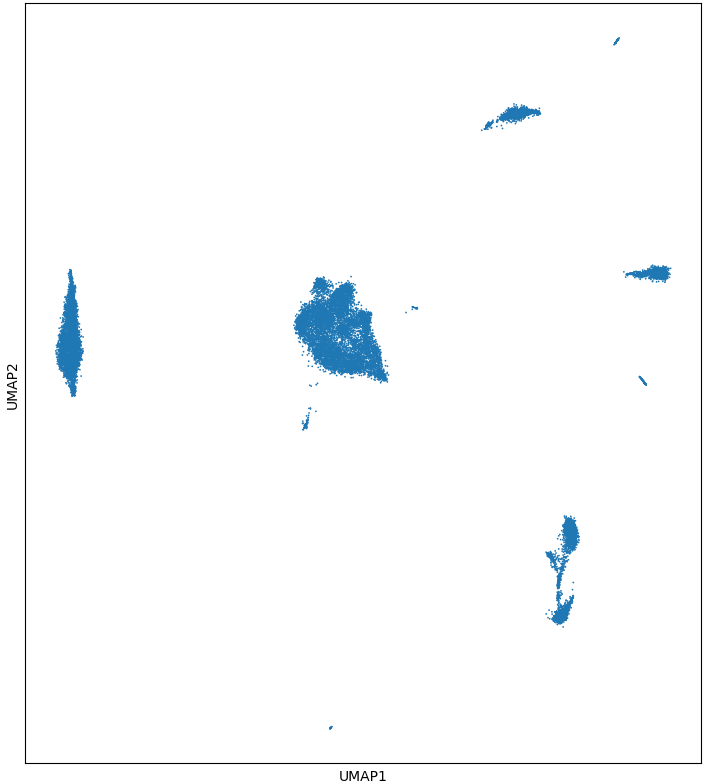
\includegraphics[height=8cm, width=15cm]{DBSCAN_cosine_eps01.png}
    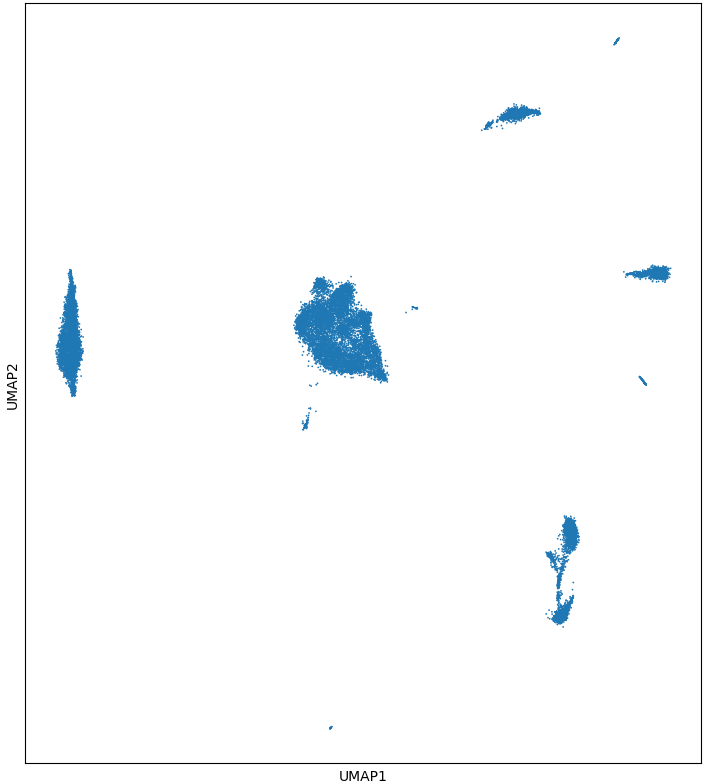
\includegraphics[width=0.7\textwidth]{DBSCAN_cosine_eps01.png}
    \caption{Параметар максималне дистанце постављен на 0.1, косинусно растојање - алгоритам је све инстанце детектовао да представљају шум}
    \label{fig:gustina1}
\end{figure}
\begin{figure}[H]
    \centering
    \captionsetup{justification=centering}
    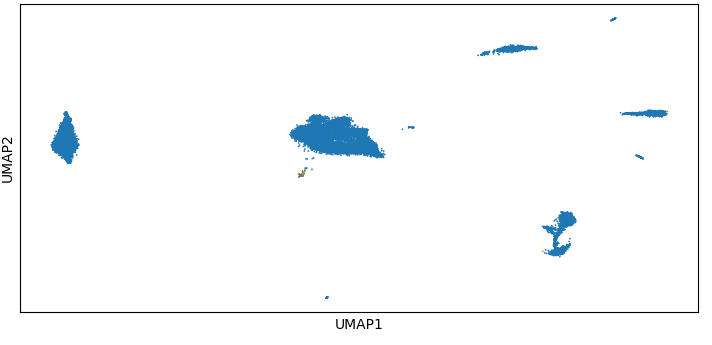
\includegraphics[width=0.7\textwidth]{DBSCAN_cosine_05.png}
    \caption{Параметар максималне дистанце постављен на 0.5, косинусно растојање - алгоритам је све скоро све инстанце детектовао као шум, док је само мањи део означен наранџастом бојом детектован као кластер}
    \label{fig:gustina2}
\end{figure}
\begin{figure}[H]
    \centering
    \captionsetup{justification=centering}
    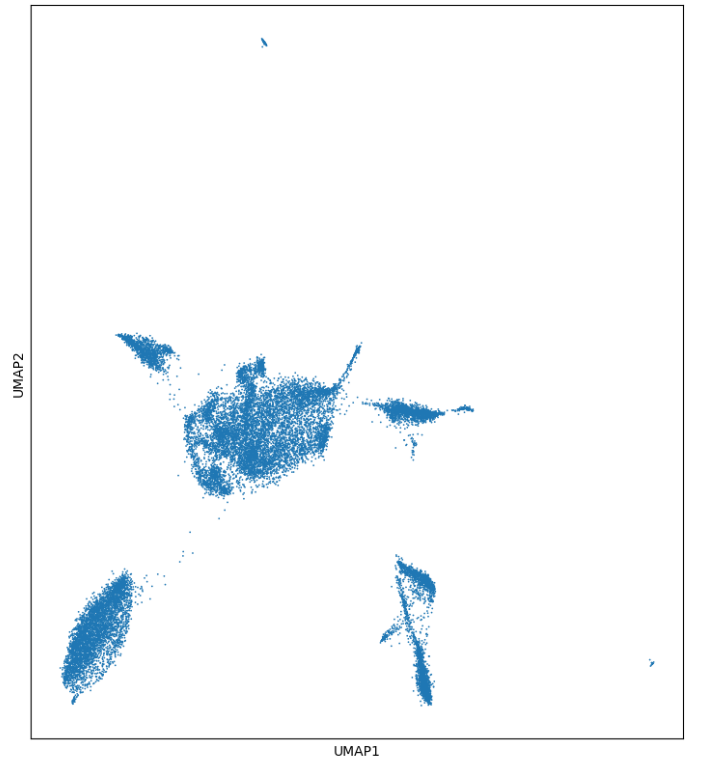
\includegraphics[width=0.7\textwidth]{dbscan_euclid.png}
    \caption{Еуклидско растојанје - независно од параметра максималне дистанце алгоритам је показивао да су све тачке шум}
    \label{fig:gustina2}
\end{figure}
\subsection{Алгоритми засновани на графовима}
\label{subsec: podnaslov7}
У кластеровању заснованом на графовима подаци су представљени као чворови унутар графа, а везе између чворова представљају сличност између свака два различита чвора. Овај концепт кластеровања се све чешће користи у биолошким, медицинским, астрономским истраживањима, као и за анализу података у пољима експресије гена и анализе структуре протеина. Кластеровање засновано на графовима се заснива на претпоставкама о присуству густих заједница унутар графа које се могу представити као густи подграфови или спектралне компоненте. Овиме се кластеровање мање ослања на претпоставке о математичкој расподели целог скупа података што може бити од велике користи јер често при обради великог скупа података, подскупови имају различите расподеле. Мана овог приступа је што захтева веће меморијске и временске ресурсе. Један од чешће коришћених алгоритама графовског кластеровања је \textbf{спектрално кластеровање}. У математици, спектрална теорија графова представља изучавање својстава графова коришћењем матрица које су им придружене тј. њихових карактеристичних полинома, сопствених вредности и сопствених вектора. \cite{spektralno} Неки од најзанимљивијих својстава представљају \textbf{матрица повезаности} и \textbf{Лапласова матрица}.
\begin{figure}[H]
    \centering
    \captionsetup{justification=centering}
    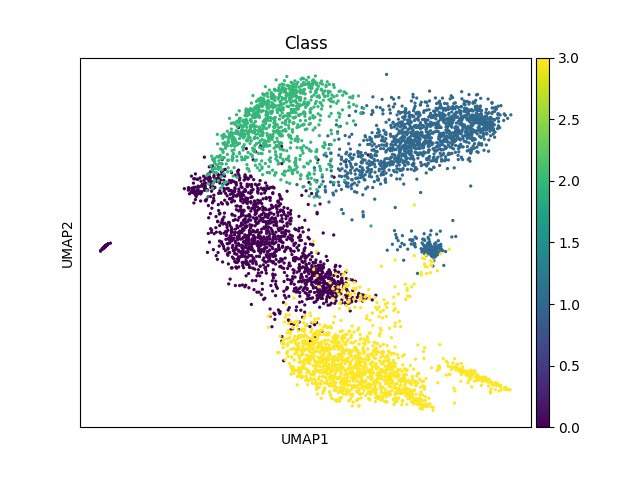
\includegraphics[width=0.6\textwidth]{spectral_l1_150.png}
    \caption{Спектрално кластеровање без Т ћелија са метриком Менхетн и са параметром број суседа постављеним на вредност 150}
    \label{fig:gustina2}
\end{figure}

Спектрално кластеровање се најчешће примењује за кластеровање података чији кластери немају конвексну или угњеждену структуру. Користе се спектрална својства Лапласове матрице како би се подаци пројектовали у нискодимензионалном простор у коме је, потом, ефикасније извршити кластеровање. Мана је што цео процес захтева О($n^3$) времена где је n број тачака скупа који кластерујемо. Два су главна корака алгоритма: формирање Лапласове матрице, а након тога примена алгоритма К-средина на сопствене векторе добијених из Лапласове матрице.
\begin{figure}[H]
    \centering
    \captionsetup{justification=centering}
    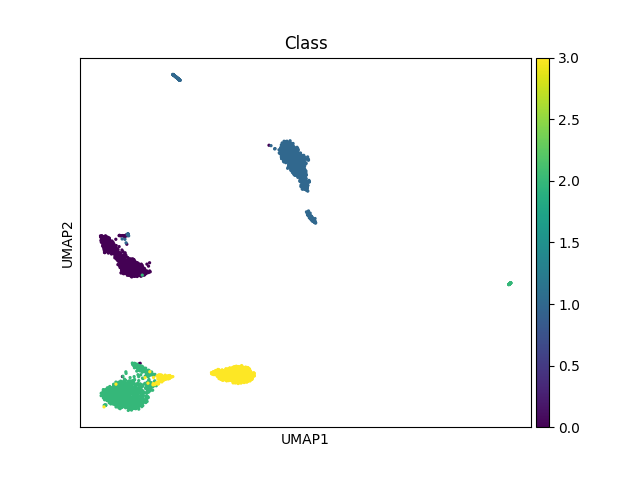
\includegraphics[width=0.7\textwidth]{spectral_cosine_90.png}
    \caption{Спектрално кластеровање без Т ћелија са Еуклидском метриком и са параметром број суседа постављеним на вредност 90}
    \label{fig:gustina2}
\end{figure}
\newpage
Приликом обраде целокупног скупа података најбоље се показало спектрално кластеровање, али са претходно израчунатом матрицом дистанци. Матрице су рачучунате уз помоћ scanpy метода neighbors, а потом су прослеђиване алгоритму кластеровања који је на основу њих груписао ћелије. Коришћењем корелационих и косинусних метрика достигнута је прецизност од скоро 80\%. Прецизност је зависила од параметра број суседа који се прослеђује методи neighbors. У сликама број 9 и 10 су приказани резултати кластеровања, као и горе поменути параметри. Прецизност кластеровања опада кад се у скуп обрађиваних података додају Т ћелије.

\begin{figure}[H]
    \centering
    \captionsetup{justification=centering}
    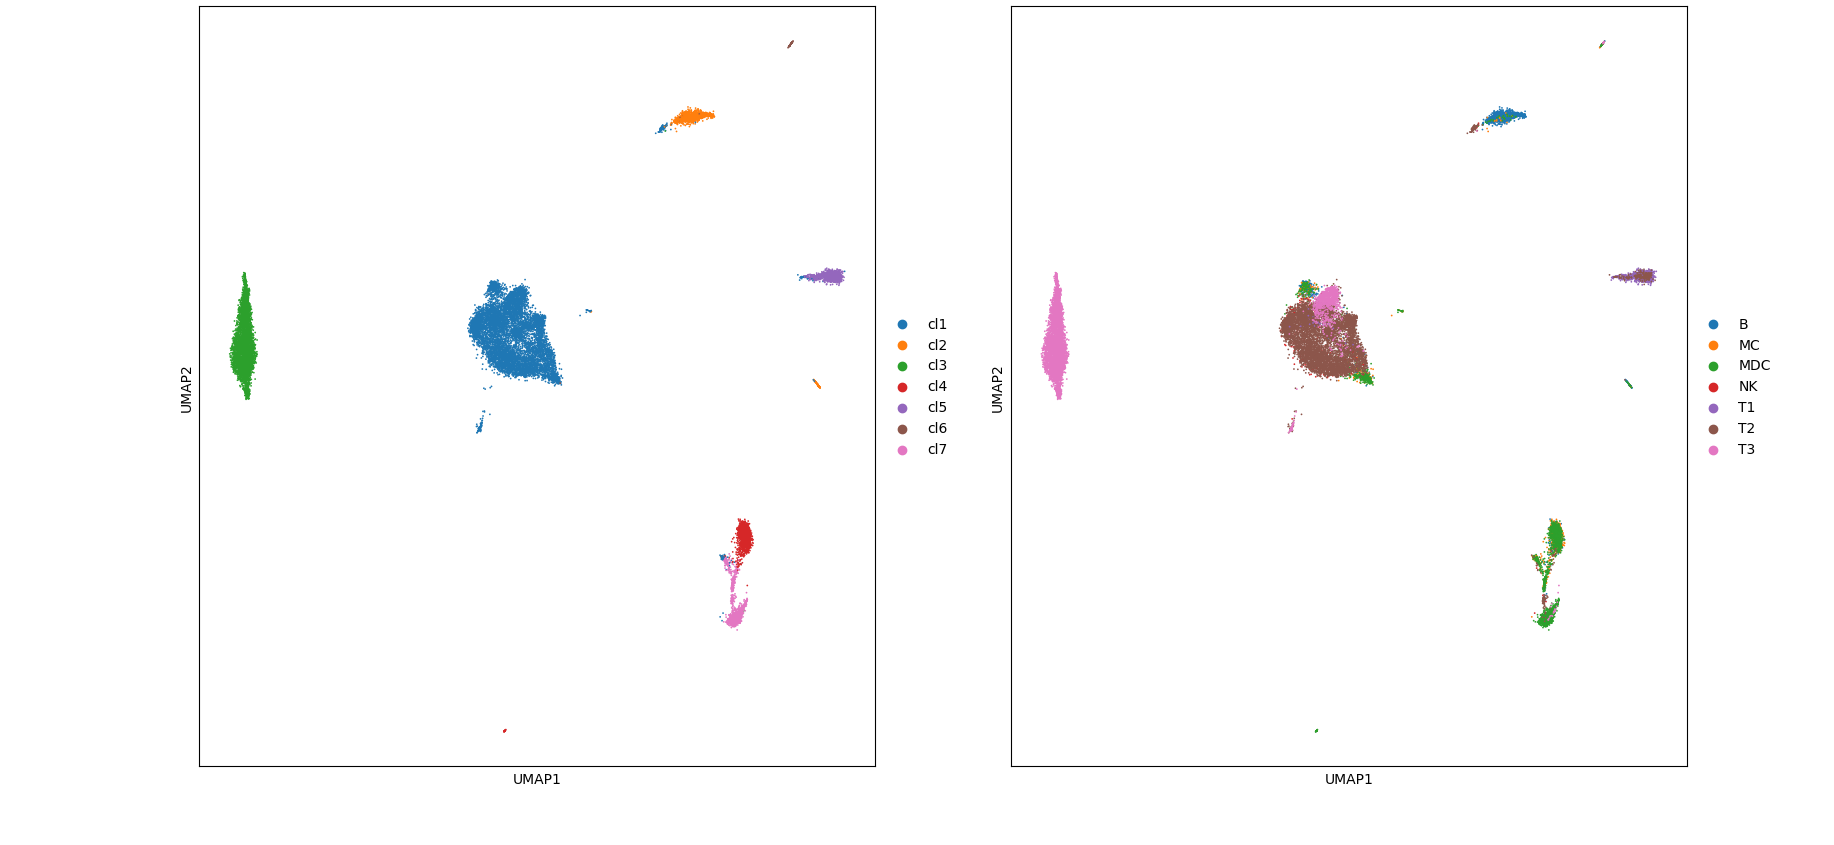
\includegraphics[width=1.1\textwidth]{all_cells_cosine_110.png}
    \caption{Спектрално кластеровање свих ћелија са косинусном метриком и са параметром број суседа постављеним на вредност 110 (лево - слика кластерованих података, десно - слика реалног распореда података)}
    \label{fig:gustina2}
\end{figure}

\begin{figure}[H]
    \centering
    \captionsetup{justification=centering}
    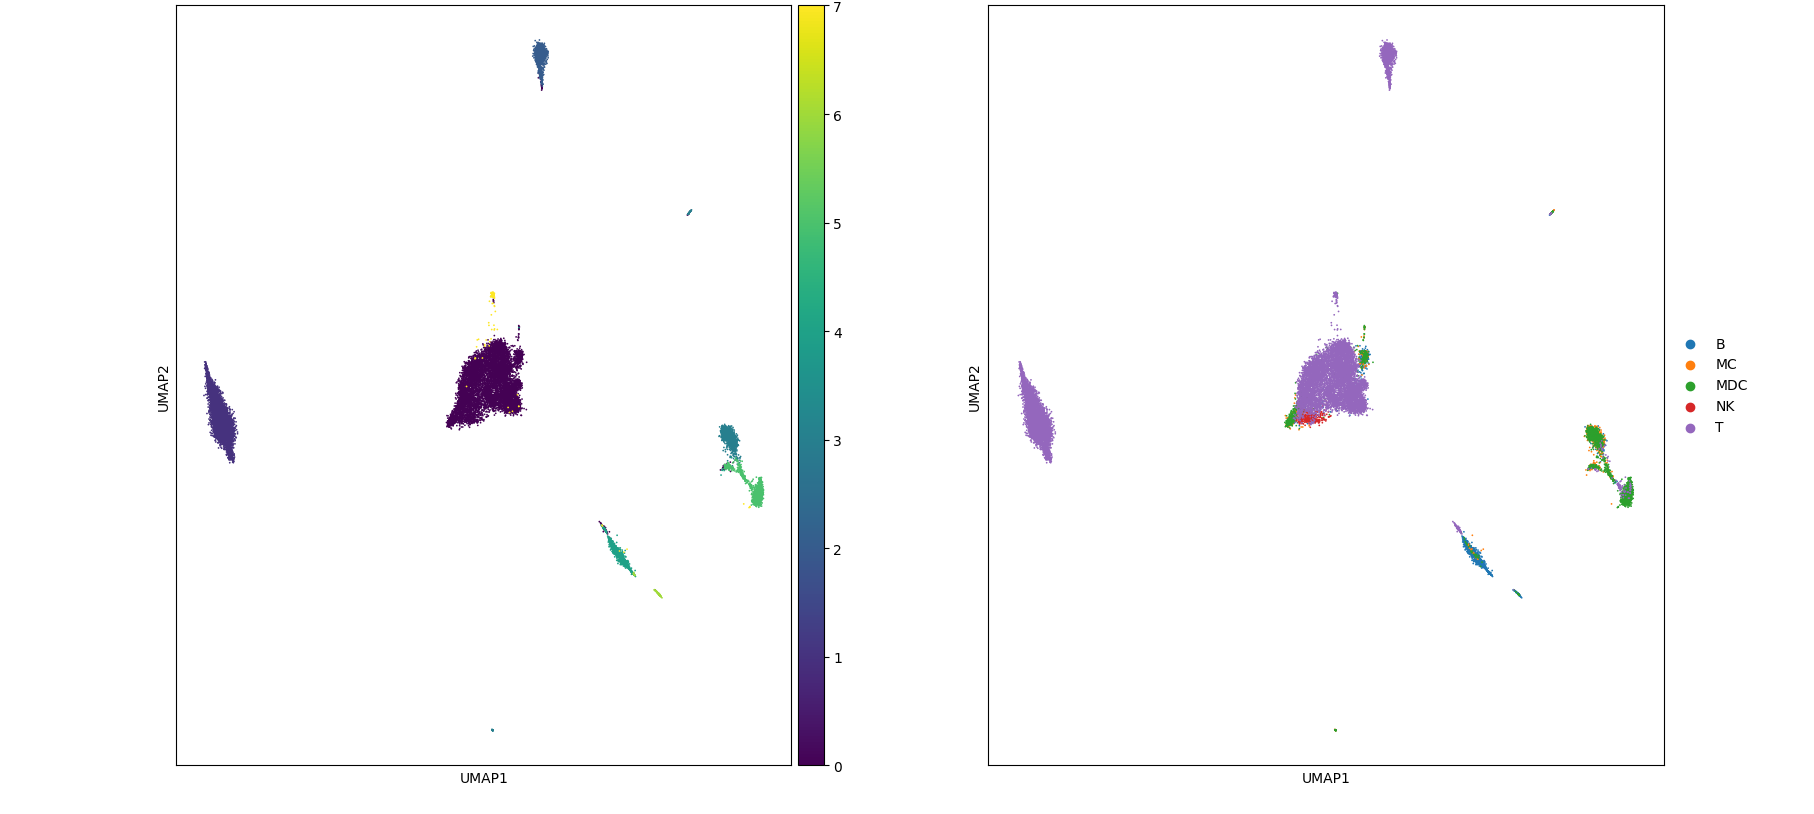
\includegraphics[width=1.1\textwidth]{All_cells_correlation_150_8cls.png}
    \caption{Спектрално кластеровање свих ћелија са корелационом метриком и са параметром број суседа постављеним на вредност 150 (лево - слика кластерованих података, десно - слика реалног распореда података)}
    \label{fig:gustina2}
\end{figure}
%\section{Резултати}
%\label{sec: naslov4}


\section{Закључак}
\label{sec: naslov5}

Идентификација типова ћелија је основни проблем анализe података методом jедноћелиjске транскриптомиjе. Последњих година су предлагане многе методе кластеровања за решавањe проблема идентификације. Међутим, већина ових метода се не могу лако генерализовати, односно дају различите резултате за различите скупове података.

За визуелизацију података је коришћена новија библиотека UMAP у циљу очувања глобалне структуре распореда ћелија. Испробаване су технике које су се у радовима из ранијих година показале најбоље. Коришћени су алгоритми К средина, DBSCAN и спектрално кластеровање, а најбоље се показао алгоритам спектралног кластеровања са различитим методама рачунања матрице дистанце. Такође су испробаване различите метрике за рачунање матрице дистанце од којих су косинусна и корелациона метрика дале најбоље резултате. Уочено је да модели где су били присутни нула гени се нису значајно разликовали од модела из којих су нула гени уклоњени.

Поред ефикасних техника кластеровања које се развијају данас, неопходне су и биолошке методе за интерпретацију резултата. Није разјашњено да ли су начин на који су кластери формирани и сличност модела добијених у оквиру оба тока рада последице параметара алгоритма или међусобних односа које ћелије имају унутар скупа података. Даљим напретком науке и развитком метода, како биолошких тако и рачунарских, очекујемо јасније резултате у пољу истраживања података у биоинформатици.

\break
\printbibliography[heading=bibnumbered]

\end{document}
